\documentclass{article}
\usepackage{mathtools}
\usepackage{amsthm}
\usepackage{listings}
\usepackage{amssymb}
\usepackage{tikz}
\usepackage{soul}
\usepackage{graphicx}
\usepackage{hyperref}
\renewcommand{\baselinestretch}{1.5}
\lstset{
  frame=none,
  xleftmargin=2pt,
  stepnumber=1,
  numbers=left,
  numbersep=5pt,
  numberstyle=\ttfamily\tiny\color[gray]{0.3},
  belowcaptionskip=\bigskipamount,
  captionpos=b,
  escapeinside={*'}{'*},
  language=haskell,
  tabsize=2,
  emphstyle={\bf},
  commentstyle=\it,
  stringstyle=\mdseries\rmfamily,
  showspaces=false,
  keywordstyle=\bfseries\rmfamily,
  columns=flexible,
  basicstyle=\small\sffamily,
  showstringspaces=false,
  morecomment=[l]\%,
}
\title{Solutions for "Relations" chapter of "How to prove it" book}
\author{
    by drets\\
}

\date{May 2017}
\newcommand{\vs}{\vspace{30pt}}
\begin{document}

\maketitle

\centerline{(make contain various errors)}

\section{Ordered Pairs and Cartesian Products}

1.

(a) $\{(p, c) \in P \times P \mid \text{the person p is a parent of c}\}$ = \{(Prince Charles, Prince William), (Prince Charles, Price Harry), \dots\}

(b) $\{(c, u) \in C \times U \mid \text{there is someone who lives in c and attends u}\}$. If you are a university student, then let x be the city you live in, and let y be the university you attend; (x, y) will then be an element of this truth set.
\vs

2.

(a) $\{(p, c) \in P \times C \mid \text{the person p lives in c city})\}$ = \{(drets, Poznan), (Prince William, London), \dots\}

(b) $\{(c, n) \in C \times \mathbb{N} \mid \text{the population of c is n}\} = \{(Poznan, 600000), (Tokyo, 13600000), \dots\}$
\vs

3.

(a) $y = x^2 - x - 2$

$\{(0, -2), (2, 0), \dots\}$

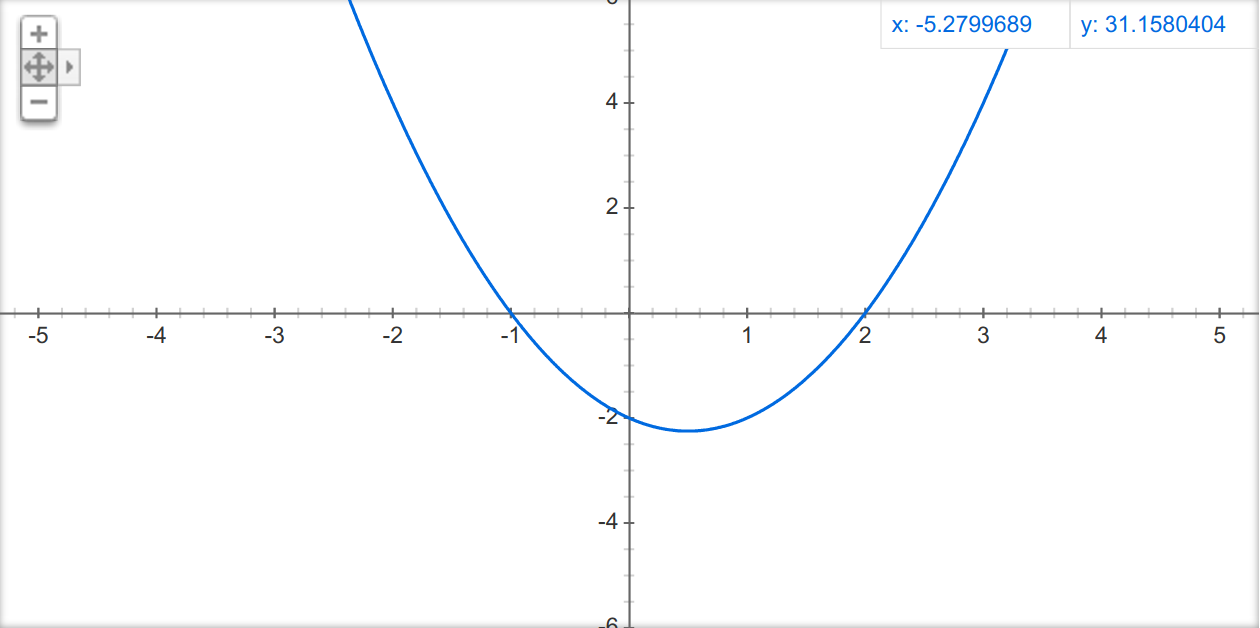
\includegraphics[width=\textwidth,height=\textheight,keepaspectratio]{misc/4_1_3_1}
\vs

(b) $y < x$

$\{(0,1), (0.1, 1.1), \dots\}$
\vs

(c) Either $y = x^2 - x - 2$ or $y = 3x - 2$

$\{(-1, 0), (0, -2), (0.666666(6),0),(2, 0), \dots\}$

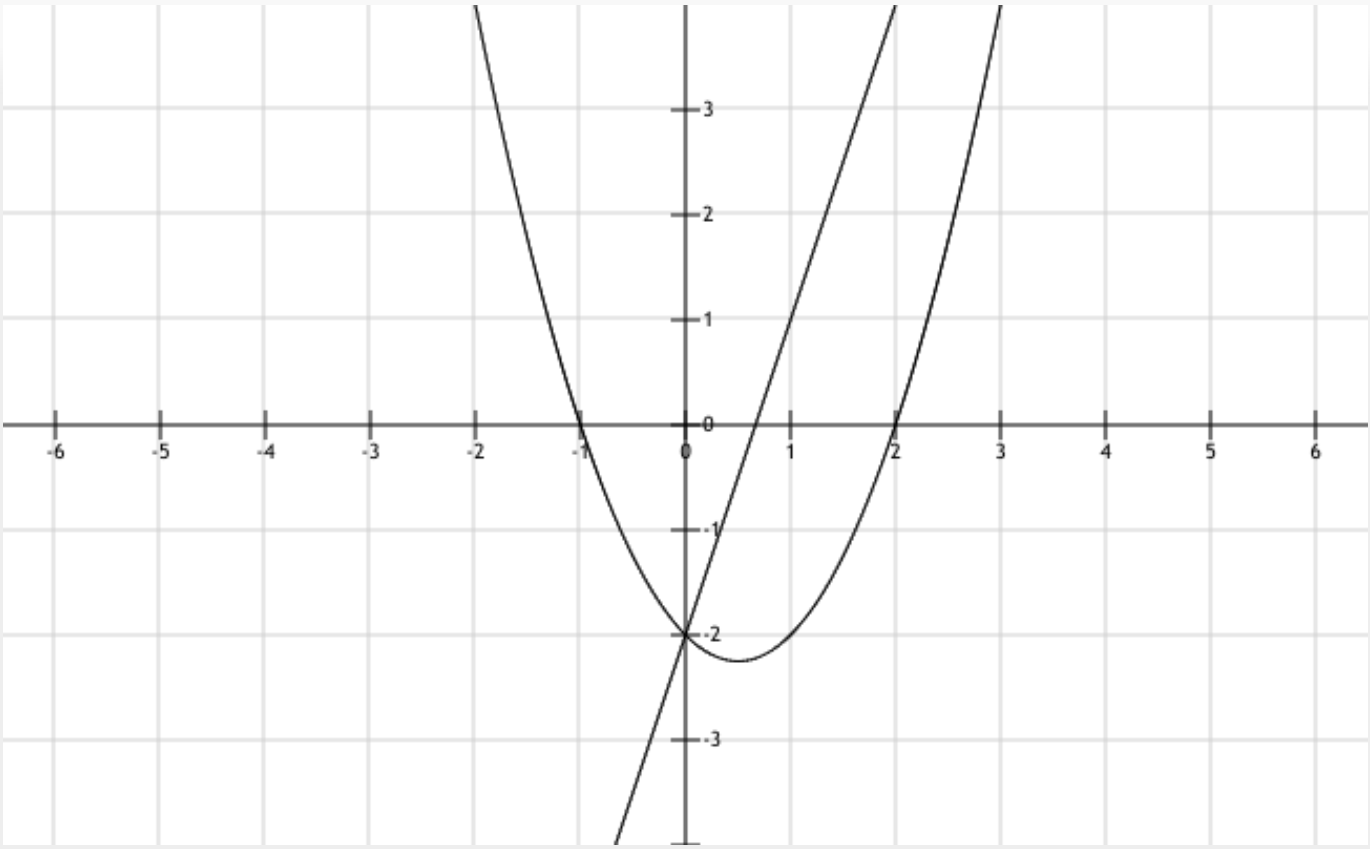
\includegraphics[width=\textwidth,height=\textheight,keepaspectratio]{misc/4_1_3_3}
\vs

(d) $y < x$, and either $y = x^2 - x - 2$ or $y = 3x - 2$

$\{(0, -2), (0.666666(6),0),(2, 0), \dots\}$

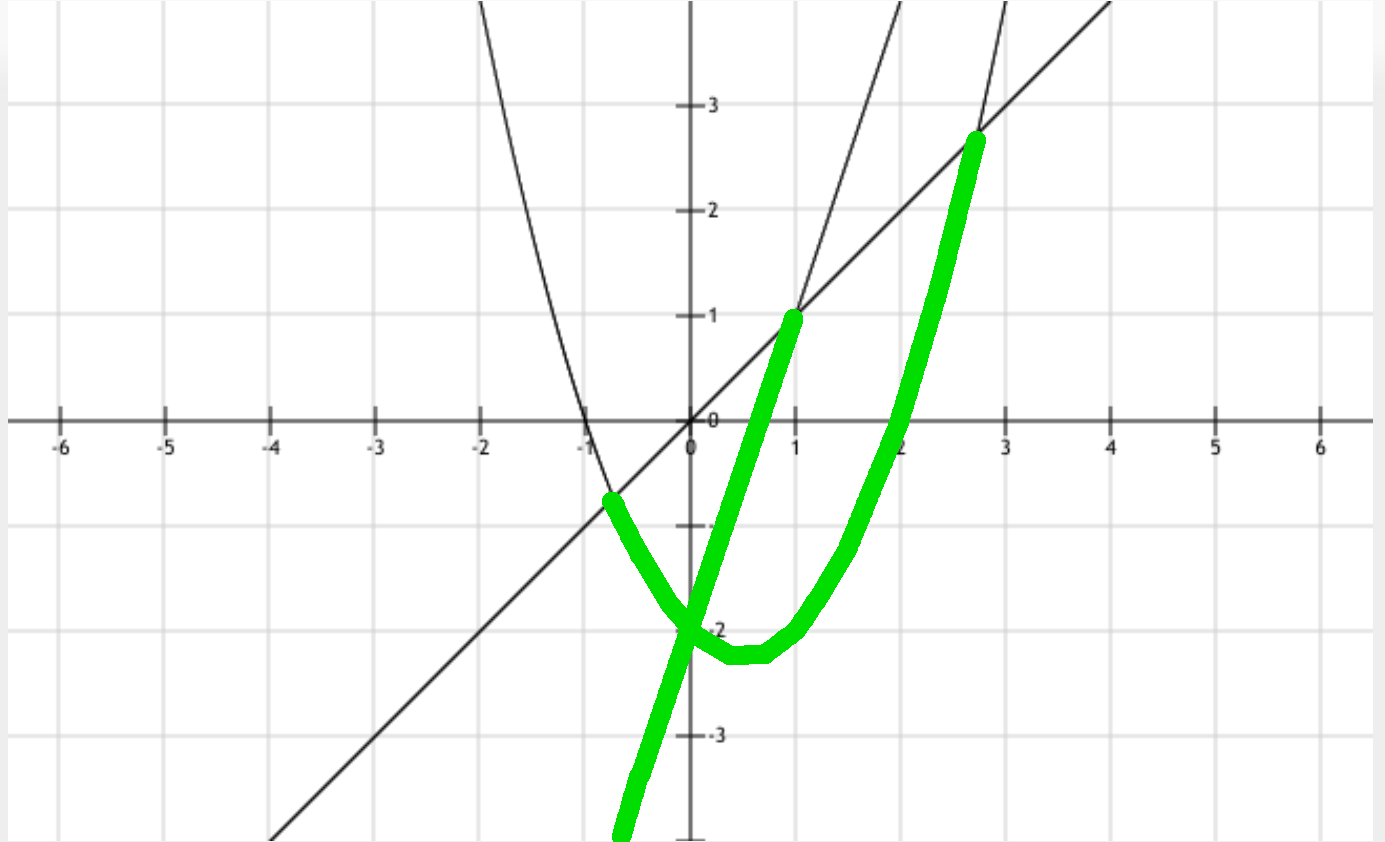
\includegraphics[width=\textwidth,height=\textheight,keepaspectratio]{misc/4_1_3_4}
\vs

4.

$A = \{1,2,3\}$

$B = \{1,4\}$

$C = \{3,4\}$

$D = \{5\}$

1) $A \times (B \cap C) = (A \times B) \cap (A \times C)$

$B \cap C = \{4\}$

$A \times (B \cap C) = \{(1,4), (2,4), (3,4)\}$

$A \times B = \{(1,1), (2,1), (3,1), (1,4), (2,4), (3,4)\}$

$A \times C = \{(1,3), (2,3), (3,3), (1,4), (2,4), (3,4)\}$

$(A \times B) \cap (A \times C) = \{(1,4), (2,4), (3,4)\}$

2) $A \times (B \cup C) = (A \times B) \cup (A \times C)$

$B \cup C = \{1,3,4\}$

$A \times (B \cup C) = \{(1, 1), (2, 1), (3, 1), (1, 3), (2, 3), (3, 3), (1, 4), (2, 4), (3, 4)\}$

$A \times B = \{(1,1), (2,1), (3,1), (1,4), (2,4), (3,4)\}$

$A \times C = \{(1,3), (2,3), (3,3), (1,4), (2,4), (3,4)\}$

$(A \times B) \cup (A \times C) = \{(1,1), (2,1), (3,1), (1,3), (2,3), (3,3), (1,4), (2,4), (3,4)\}$

3) $(A \times B) \cap (C \times D) = (A \cap C) \times (B \cap D)$

$A \times B = \{(1,1), (2,1), (3,1), (1,4), (2,4), (3,4)\}$

$C \times D = \{(3,5), (4,5)\}$

$(A \times B) \cap (C \times D) = \varnothing$

$A \cap C = {3}$

$B \cap D = \varnothing$

$(A \cap C) \times (B \cap D) = \varnothing$

4) $(A \times B) \cup (C \times D) \subseteq (A \cup C) \times (B \cup D)$

$A \times B = \{(1,1), (2,1), (3,1), (1,4), (2,4), (3,4)\}$

$C \times D = \{(3,5), (4,5)\}$

$(A \times B) \cup (C \times D) = \{(1,1), (2,1), (3,1), (1,4), (2,4), (3,4), (3,5), (4,5)\}$

$A \cup C = \{1,2,3,4\}$

$B \cup D = \{1,4,5\}$

$(A \cup C) \times (B \cup D) = \{(1,1),(2,1),(3,1),(4,1),(1,4),(2,4),(3,4),(4,4),(1,5),(2,5),(3,5),(4,5)\}$

5) $A \times \varnothing = \varnothing \times A = \varnothing$

$A \times \varnothing = \{1,2,3\} \times \varnothing = \varnothing$

$\varnothing \times A = \varnothing \times \{1,2,3\} =  \varnothing$
\vs

5.

$A \times (B \cup C) = (A \times B) \cup (A \times C)$

1)

\centerline{
  \begin{tabular}{l l}
  \textit{Givens} & \textit{Goal} \\
  $p \in A \times (B \cup C)$ & $p \in (A \times B) \cup (A \times C)$ \\
  \end{tabular}}
\vs

\centerline{
  \begin{tabular}{l l}
  \textit{Givens} & \textit{Goal} \\
    $x \in A$ & $p \in (A \times B) \cup (A \times C)$ \\
    $y \in B \lor y \in C$ & \\
  \end{tabular}}
\vs

\centerline{
  \begin{tabular}{l l}
  \textit{Givens} & \textit{Goal} \\
   $x \in A$ & $p \in (A \times B) \cup (A \times C)$ \\
   $y \in B \lor y \in C$ & \\
 \end{tabular}}
\vs

Case 1.

\centerline{
  \begin{tabular}{l l}
  \textit{Givens} & \textit{Goal} \\
   $x \in A$ & $p \in (A \times B) \cup (A \times C)$ \\
   $y \in B$ & \\
 \end{tabular}}
\vs

Case 2.

\centerline{
  \begin{tabular}{l l}
  \textit{Givens} & \textit{Goal} \\
   $x \in A$ & $p \in (A \times B) \cup (A \times C)$ \\
   $y \in C$ & \\
 \end{tabular}}
\vs

2)

\centerline{
  \begin{tabular}{l l}
  \textit{Givens} & \textit{Goal} \\
  $p \in (A \times B) \cup (A \times C)$ & $p \in A \times (B \cup C)$ \\
  \end{tabular}}
\vs

Case 1.

\centerline{
  \begin{tabular}{l l}
    \textit{Givens} & \textit{Goal} \\
    $x \in A$ & $x \in A \land (y \in B \lor y \in C)$ \\
    $y \in B$
  \end{tabular}}
\vs

Case 2.

\centerline{
  \begin{tabular}{l l}
  \textit{Givens} & \textit{Goal} \\
    $x \in A$ & $x \in A \land (y \in B \lor y \in C)$ \\
    $y \in C$
  \end{tabular}}
\vs

\textit{Proof of 2.} Let p be an arbitrary element of $A \times (B \cup C)$. Then by definition of Cartesian
product, p must be an ordered pair whose first coordinate is an element of A and second coordinate is an element of $B \cup C$. In other words, $p = (x, y)$ for some $x \in A$ and $y \in B \cup C$. Since $y \in B \cup C$, $y \in B$ or $y \in C$.

Case 1. $y \in B$. Since $x \in A$ and $y \in B$, $p = (x, y) \in A \times B$. Thus, $p \in (A \times B) \cup (A \times C)$

Case 2. $y \in C$. Since $x \in A$ and $y \in C$, $p = (x, y) \in A \times C$. Thus, $p \in (A \times B) \cup (A \times C)$

Since p was an arbitrary element of $A \times (B \cup C)$, it follows that $A \times (B \cup C) \subseteq (A \times B) \cup (A \times C)$.


Now let p be an arbitrary element of $p \in (A \times B) \cup (A \times C)$. Then $p \in A \times B$ or $p \in A \times C$.

Case 1. $p \in A \times B$. Then $p = (x, y)$ for some $x \in A$ and $y \in B$. Thus, $x \in A \lor (y \in B \lor y \in C)$. Therefore, $p \in A \times (B \cup C)$

Case 2. $p \in A \times C$. Then $p = (x, y)$ for some $x \in A$ and $y \in C$. Thus, $x \in A \lor (y \in B \lor y \in C)$. Therefore, $p \in A \times (B \cup C)$.

Since p was an arbitrary element of $p \in (A \times B) \cup (A \times C)$, it follows that $(A \times B) \cup (A \times C) \subseteq A \times (B \cup C)$, so $(A \times B) \cup (A \times C) = A \times (B \cup C)$
\vs

$(A \times B) \cap (C \times D) = (A \cap C) \times (B \cap D)$

1)

\centerline{
  \begin{tabular}{l l}
  \textit{Givens} & \textit{Goal} \\
    $p \in (A \times B) \cap (C \times D)$ & $p \in (A \cap C) \times (B \cap D)$ \\
  \end{tabular}}
\vs

\centerline{
  \begin{tabular}{l l}
  \textit{Givens} & \textit{Goal} \\
    $p \in A \times B$ & $p \in (A \cap C) \times (B \cap D)$ \\
    $p \in C \times D$ & \\
  \end{tabular}}
\vs

\centerline{
  \begin{tabular}{l l}
  \textit{Givens} & \textit{Goal} \\
    $x \in A$ & $p \in (A \cap C) \times (B \cap D)$ \\
    $y \in B$ & \\
    $x \in C$ & \\
    $y \in D$ & \\
  \end{tabular}}
\vs

2)

\centerline{
  \begin{tabular}{l l}
  \textit{Givens} & \textit{Goal} \\
    $p \in (A \cap C) \times (B \cap D)$ & $p \in (A \times B) \cap (C \times D)$ \\
  \end{tabular}}
\vs

\centerline{
  \begin{tabular}{l l}
  \textit{Givens} & \textit{Goal} \\
    $x \in A \cap C$ & $p \in (A \times B) \cap (C \times D)$ \\
    $y \in B \cap D$ & \\
  \end{tabular}}
\vs

\textit{Proof of 3}

Let $(x, y)$ be an arbitrary element of $(A \times B) \cap (C \times D)$. Then $(x, y) \in A \times B$ and $(x, y) \in C \times D$. Then $x \in A$ and $x \in C$, and $y \in B$ and $y \in D$. Therefore $(x, y) \in (A \cap C) \times (B \cap D)$. Since $(x, y)$ was an arbitrary element of $(A \times B) \cap (C \times D)$, it follows that
$(A \times B) \cap (C \times D) \subseteq (A \cap C) \times (B \cap D)$

Now let $(x, y)$ be an arbitrary element of $(A \cap C) \times (B \cap D)$. Then $x \in A$ and $x \in C$, and $y \in B$ and $y \in D$. Therefore $(x, y) \in (A \times B) \cap (C \times D)$. Since $(x, y)$ was an arbitrary element of $(A \cap C) \times (B \cap D)$, it follows that $(A \cap C) \times (B \cap D) \subseteq (A \times B) \cap (C \times D)$, so $(A \times B) \cap (C \times D) = (A \cap C) \times (B \cap D)$.
\vs

6. The cases are not exhaustive.
\vs

7. If A has m elements and B has n elements, $A \times B$ have $m * n$ elements.
\vs

8.

$A \times (B \setminus C) = (A \times B) \setminus (A \times C)$
\vs

1)

\centerline{
  \begin{tabular}{l l}
  \textit{Givens} & \textit{Goal} \\
    $p \in A \times (B \setminus C)$ & $p \in (A \times B) \setminus (A \times C)$ \\
  \end{tabular}}
\vs

\centerline{
  \begin{tabular}{l l}
  \textit{Givens} & \textit{Goal} \\
    $x \in A$ & $p \in A \times B \land \neg (p \in A \times C)$ \\
    $y \in B$ & \\
    $y \notin C$ & \\
  \end{tabular}}
\vs

\centerline{
  \begin{tabular}{l l}
  \textit{Givens} & \textit{Goal} \\
    $x \in A$ & $x \in A \land y \in B \land \neg (x \in A \land y \in C)$ \\
    $y \in B$ & \\
    $y \notin C$ & \\
  \end{tabular}}
\vs

\centerline{
  \begin{tabular}{l l}
  \textit{Givens} & \textit{Goal} \\
    $x \in A$ & $x \in A \land y \in B \land (x \notin A \lor y \notin C)$ \\
    $y \in B$ & \\
    $y \notin C$ & \\
  \end{tabular}}
\vs

2)

\centerline{
  \begin{tabular}{l l}
  \textit{Givens} & \textit{Goal} \\
    $p \in (A \times B) \setminus (A \times C)$ & $p \in A \times (B \setminus C)$ \\
  \end{tabular}}
\vs

\centerline{
  \begin{tabular}{l l}
  \textit{Givens} & \textit{Goal} \\
    $x \in A \land y \in B \land (x \notin A \lor y \notin C)$ & $x \in A \land y \in B \land y \notin C$ \\
  \end{tabular}}
\vs

Case 1.

\centerline{
  \begin{tabular}{l l}
  \textit{Givens} & \textit{Goal} \\
    $x \in A \land y \in B \land y \notin C$ & $x \in A \land y \in B \land y \notin C$ \\
  \end{tabular}}
\vs

Case 2.

\centerline{
  \begin{tabular}{l l}
  \textit{Givens} & \textit{Goal} \\
    $x \in A \land y \in B \land x \notin A$ & $x \in A \land y \in B \land y \notin C$ \\
  \end{tabular}}
\vs

\centerline{
  \begin{tabular}{l l}
  \textit{Givens} & \textit{Goal} \\
    $x \in A \land y \in B$ & $x \in A$ \\
  \end{tabular}}
\vs

\textbf{Theorem.} $A \times (B \setminus C) = (A \times B) \setminus (A \times C)$

\textit{Proof.} Let $(x, y)$ be an arbitrary element of $A \times (B \setminus C)$. Then $x \in A$, $y \in B$ and $y \notin C$. Thus $x \in A \land y \in B \land (x \notin A \lor y \notin C)$. Therefore, $(x, y) \in (A \times B) \setminus (A \times C)$. Since $(x, y)$ was an arbitrary element of $A \times (B \setminus C)$, it follows that $A \times (B \setminus C) \subseteq (A \times B) \setminus (A \times C)$.

Now let $(x, y)$ be arbitrary element of $(A \times B) \setminus (A \times C)$. Then $x \in A \land y \in B \land (x \notin A \lor y \notin C)$.

Case 1. $x \notin A$. $x \notin A$ contradicts to $x \in A$.

Case 2. $y \notin C$. Then $x \in A$ and $y \in B$ and $y \notin C$. Therefore, $(x, y) \in A \times (B \setminus C)$

Since $(x, y)$ was an arbitrary element of $(A \times B) \setminus (A \times C)$, it follows that $(A \times B) \setminus (A \times C) \subseteq A \times (B \setminus C)$, so $(A \times B) \setminus (A \times C) = A \times (B \setminus C)$.
\vs

9. $(A \times B) \setminus (C \times D) = [A \times (B \setminus D)] \cup [(A \setminus C) \times B]$

1)

\centerline{
  \begin{tabular}{l l}
  \textit{Givens} & \textit{Goal} \\
    $(x,y) \in (A \times B) \setminus (C \times D)$ & $(x \in A \land y \in B \land y \notin D) \lor (x \in A \land x \notin C \land y \in B)$ \\
  \end{tabular}}
\vs

$(x,y) \in (A \times B) \setminus (C \times D)$

$x \in A \land y \in B \land (x \notin C \lor y \notin D$

\centerline{
  \begin{tabular}{l l}
  \textit{Givens} & \textit{Goal} \\
    $x \in A \land y \in B \land (x \notin C \lor y \notin D)$ & $(x, y) \in [A \times (B \setminus D)] \cup [(A \setminus C) \times B]$ \\
  \end{tabular}}
\vs

$(x, y) \in [A \times (B \setminus D)] \cup [(A \setminus C) \times B]$

$(x \in A \land y \in B \land y \notin D) \lor (x \in A \land x \notin C \land y \in B)$

\centerline{
  \begin{tabular}{l l}
  \textit{Givens} & \textit{Goal} \\
    $x \in A \land y \in B \land (x \notin C \lor y \notin D)$ & $(x \in A \land y \in B \land y \notin D) \lor (x \in A \land x \notin C \land y \in B)$ \\
  \end{tabular}}
\vs

\centerline{
  \begin{tabular}{l l}
  \textit{Givens} & \textit{Goal} \\
    $x \in A \land y \in B \land (x \notin C \lor y \notin D)$ & $x \in A \land y \in B \land (x \notin C \lor y \notin D)$ \\
  \end{tabular}}
\vs

2)

\centerline{
  \begin{tabular}{l l}
  \textit{Givens} & \textit{Goal} \\
    $(x, y) \in [A \times (B \setminus D)] \cup [(A \setminus C) \times B]$ & $(x,y) \in (A \times B) \setminus (C \times D)$ \\
  \end{tabular}}
\vs

\centerline{
  \begin{tabular}{l l}
  \textit{Givens} & \textit{Goal} \\
    $x \in A \land y \in B \land (x \notin C \lor y \notin D)$ & $x \in A \land y \in B \land (x \notin C \lor y \notin D)$ \\
  \end{tabular}}
\vs

\textbf{Theorem.} $(A \times B) \setminus (C \times D) = [A \times (B \setminus D)] \cup [(A \setminus C) \times B]$

\textit{Proof.} Let (x, y) be an arbitrary element of $(A \times B) \setminus (C \times D)$. Then $x \in A \land y \in B \land (x \notin C \lor y \notin D)$ which is equivalent to $(x \in A \land y \in B \land y \notin D) \lor (x \in A \land x \notin C \land y \in B)$. Thus $(x,y) \in [A \times (B \setminus D)] \cup [(A \setminus C) \times B]$. Since $(x, y)$ was an arbitrary element of $(A \times B) \setminus (C \times D)$, it follows that $(A \times B) \setminus (C \times D) \subseteq [A \times (B \setminus D)] \cup [(A \setminus C) \times B]$.

Now let (x, y) be an arbitrary element of $[A \times (B \setminus D)] \cup [(A \setminus C) \times B]$. Then $(x \in A \land y \in B \land y \notin D) \lor (x \in A \land x \notin C \land y \in B)$ which is equivalent to $x \in A \land y \in B \land (x \notin C \lor y \notin D)$. Thus $(x,y) \in (A \times B) \setminus (C \times D)$. Since $(x, y)$ was an arbitrary element of $[A \times (B \setminus D)] \cup [(A \setminus C) \times B]$, it follows that $[A \times (B \setminus D)] \cup [(A \setminus C) \times B] \subseteq (A \times B) \setminus (C \times D)$, so $(A \times B) \setminus (C \times D) = [A \times (B \setminus D)] \cup [(A \setminus C) \times B]$.
\vs

10. If $A \times B \cap C \times D = \varnothing$ then $A \cap B = \varnothing$ or $B \cap D = \varnothing$

\centerline{
  \begin{tabular}{l l}
  \textit{Givens} & \textit{Goal} \\
    $A \times B \cap C \times D = \varnothing$ & $A \cap C = \varnothing \lor B \cap D = \varnothing$ \\
  \end{tabular}}
\vs

\centerline{
  \begin{tabular}{l l}
  \textit{Givens} & \textit{Goal} \\
    $p \notin A \times B \cap C \times D$ & $A \cap C = \varnothing \lor B \cap D = \varnothing$ \\
  \end{tabular}}
\vs

$p \notin A \times B \cap C \times D$

$\neg (x \in A \land y \in B \land x \in C \land y \in D)$

$x \notin A \lor x \notin C \lor y \notin B \lor y \notin D$

\centerline{
  \begin{tabular}{l l}
  \textit{Givens} & \textit{Goal} \\
    $x \notin A \lor x \notin C \lor y \notin B \lor y \notin D$ & $x \notin A \cap C \lor y \notin B \cap D$ \\
  \end{tabular}}
\vs

\centerline{
  \begin{tabular}{l l}
  \textit{Givens} & \textit{Goal} \\
    $x \notin A \lor x \notin C \lor y \notin B \lor y \notin D$ & $x \notin A \lor x \notin C \lor y \notin B \lor y \notin D$ \\
  \end{tabular}}
\vs

\textbf{Theorem.} If $A \times B \cap C \times D = \varnothing$ then either $A \cap B = \varnothing$ or $B \cap D = \varnothing$.

\textit{Proof.} Suppose $A \times B \cap C \times D = \varnothing$. Then $(x, y) \notin A \times B \cap C \times D$. Therefore, $x \notin A \lor x \notin C \lor y \notin B \lor y \notin D$. Then

$A \cap C = \varnothing \lor B \cap D = \varnothing$

$x \notin A \cap C \lor y \notin B \cap D$

$x \notin A \lor x \notin C \lor y \notin B \lor y \notin D$

Therefore, if $A \times B \cap C \times D = \varnothing$ then either $A \cap B = \varnothing$ or $B \cap D = \varnothing$.
\vs

11.

(a)

$\cup_{i \in I}(A_i \times B_i) \subseteq (\cup_{i \in I}A_i) \times (\cup_{i \in I}B_i)$

\centerline{
  \begin{tabular}{l l}
  \textit{Givens} & \textit{Goal} \\
    $p \in \cup_{i \in I}(A_i \times B_i)$ & $p \in (\cup_{i \in I}A_i) \times (\cup_{i \in I}B_i)$ \\
  \end{tabular}}
\vs

\centerline{
  \begin{tabular}{l l}
  \textit{Givens} & \textit{Goal} \\
    $\exists i (i \in I \land p \in A_i \times B_i)$ & $p \in (\cup_{i \in I}A_i) \times (\cup_{i \in I}B_i)$ \\
  \end{tabular}}
\vs

\centerline{
  \begin{tabular}{l l}
  \textit{Givens} & \textit{Goal} \\
    $i \in I$ & $x \in (\cup_{i \in I}A_i) \land y \in (\cup_{i \in I}B_i)$ \\
    $p \in A_i \times B_i$ & \\
  \end{tabular}}
\vs

\centerline{
  \begin{tabular}{l l}
  \textit{Givens} & \textit{Goal} \\
    $i \in I$ & $\exists (i \in I \land x \in A_i) \land \exists (i \in I \land y \in B_i)$ \\
    $x \in A_i$ & \\
    $y \in B_i$ & \\
  \end{tabular}}
\vs

\textbf{Theorem.} $\cup_{i \in I}(A_i \times B_i) \subseteq (\cup_{i \in I}A_i) \times (\cup_{i \in I}B_i)$.

\textit{Proof.} Let p be an arbitrary. Suppose $p \in \cup_{i \in I}(A_i \times B_i)$. Let choose some i such that $i \in I$ and $p \in A_i \times B_i$. Then by definition of Cartesian product $x \in A_i$ and $y \in B_i$. Since $i \in I$ and $x \in A_i$, $x \in (\cup_{i \in I}A_i)$. Since $i \in I$ and $y \in B_i$, $y \in (\cup_{i \in I}B_i)$. Since $x \in (\cup_{i \in I}A_i)$ and $y \in (\cup_{i \in I}B_i)$, $p \in (\cup_{i \in I}A_i) \times (\cup_{i \in I}B_i)$. Since p was an arbitrary, $\cup_{i \in I}(A_i \times B_i) \subseteq (\cup_{i \in I}A_i) \times (\cup_{i \in I}B_i)$.
\vs

(b)

$\forall (i, j) \in I \times I (C_{(i, j)} = A_i \times B_j \land P = I \times I)$

\centerline{
  \begin{tabular}{l l}
  \textit{Givens} & \textit{Goal} \\
    $\forall (i, j) \in I \times I (C_{(i, j)} = A_i \times B_j \land P = I \times I)$ & $\cup_{p \in P}C_p = (\cup_{i \in I} A_i) \times (\cup_{i \in I} B_i)$ \\
  \end{tabular}}
\vs

1)

\centerline{
  \begin{tabular}{l l}
  \textit{Givens} & \textit{Goal} \\
    $\forall (i, j) \in I \times I (C_{(i, j)} = A_i \times B_j \land P = I \times I)$ & $t \in (\cup_{i \in I} A_i) \times (\cup_{i \in I} B_i)$ \\
    $t \in \cup_{p \in P}C_p$ & \\
  \end{tabular}}
\vs

\centerline{
  \begin{tabular}{l l}
  \textit{Givens} & \textit{Goal} \\
    $\forall (i, j) \in I \times I (C_{(i, j)} = A_i \times B_j \land P = I \times I)$ & $t \in (\cup_{i \in I} A_i) \times (\cup_{i \in I} B_i)$ \\
    $\exists p (p \in P \land t \in C_p)$ & \\
  \end{tabular}}
\vs

\centerline{
  \begin{tabular}{l l}
  \textit{Givens} & \textit{Goal} \\
    $\forall (i, j) \in I \times I (C_{(i, j)} = A_i \times B_j \land P = I \times I)$ & $t \in (\cup_{i \in I} A_i) \times (\cup_{i \in I} B_i)$ \\
    $(i,i) \in I \times I \land t \in C_{(i,i)}$ & \\
  \end{tabular}}
\vs

\centerline{
  \begin{tabular}{l l}
  \textit{Givens} & \textit{Goal} \\
    $C_{(i, i)} = A_i \times B_i$ & $t \in (\cup_{i \in I} A_i) \times (\cup_{i \in I} B_i)$ \\
    $t \in C_{(i,i)}$ & \\
  \end{tabular}}
\vs

\centerline{
  \begin{tabular}{l l}
  \textit{Givens} & \textit{Goal} \\
    $t \in A_i \times B_i$ & $t \in (\cup_{i \in I} A_i) \times (\cup_{i \in I} B_i)$ \\
  \end{tabular}}
\vs

\centerline{
  \begin{tabular}{l l}
  \textit{Givens} & \textit{Goal} \\
    $x \in A_i$ & $x \in (\cup_{i \in I} A_i) \land y \in (\cup_{i \in I} B_i)$ \\
    $y \in B_i$ & \\
  \end{tabular}}
\vs

2)

\centerline{
  \begin{tabular}{l l}
  \textit{Givens} & \textit{Goal} \\
    $\forall (i, j) \in I \times I (C_{(i, j)} = A_i \times B_j \land P = I \times I)$ &  $t \in \cup_{p \in P}C_p$ \\
    $t \in (\cup_{i \in I} A_i) \times (\cup_{i \in I} B_i)$ & \\
  \end{tabular}}
\vs

\centerline{
  \begin{tabular}{l l}
  \textit{Givens} & \textit{Goal} \\
    $\forall (i, j) \in I \times I (C_{(i, j)} = A_i \times B_j \land P = I \times I)$ & $\exists p (p \in P \land t \in C_p)$ \\
    $\exists i (i \in I \land x \in  A_i)$ & \\
    $\exists i (i \in I \land y \in  B_i)$ & \\
  \end{tabular}}
\vs

\centerline{
  \begin{tabular}{l l}
  \textit{Givens} & \textit{Goal} \\
    $\forall (i, j) \in I \times I (C_{(i, j)} = A_i \times B_j \land P = I \times I)$ & $\exists p (p \in P \land t \in C_p)$ \\
    $(i,j) \in I \times I$ & \\
    $x \in  A_i$ & \\
    $y \in  B_j$ & \\
  \end{tabular}}
\vs

\centerline{
  \begin{tabular}{l l}
  \textit{Givens} & \textit{Goal} \\
    $C_{(i, j)} = A_i \times B_j$ & $\exists p (p \in P \land t \in C_p)$ \\
    $(i,j) \in I \times I$ & \\
    $P = I \times I$ & \\
    $t = (x, y)$ & \\
    $x \in  A_i$ & \\
    $y \in  B_j$ & \\
  \end{tabular}}
\vs

\centerline{
  \begin{tabular}{l l}
  \textit{Givens} & \textit{Goal} \\
    $C_{(i, j)} = A_i \times B_j$ & $\exists p (p \in P \land t \in C_p)$ \\
    $(i,j) \in P$ & \\
    $t \in  A_i \times B_j$ & \\
  \end{tabular}}
\vs

\centerline{
  \begin{tabular}{l l}
  \textit{Givens} & \textit{Goal} \\
    $t \in  C_{(i,j)}$ & $\exists p (p \in P \land t \in C_p)$ \\
    $(i,j) \in P$ & \\
  \end{tabular}}
\vs

\textbf{Theorem.} Suppose $\forall (i, j) \in I \times I (C_{(i, j)} = A_i \times B_j \land P = I \times I)$. Then $\cup_{p \in P}C_p = (\cup_{i \in I} A_i) \times (\cup_{i \in I} B_i)$.

\textit{Proof.} Let t be an arbitrary element of $\cup_{p \in P}C_p$. Then we can choose some p such that $p \in I \times I$ and $t \in C_p$. Since $\forall (i, j) \in I \times I (C_{(i, j)} = A_i \times B_j \land P = I \times I)$, then in particular $C_p = A_i \times B_j$ and $P = I \times I$. Since $t \in C_p$ and $C_p = A_i \times B_j$, $t \in A_i \times B_j$. Since $t \in A_i \times B_i$, $x \in A_i$ and $y \in B_i$. Since $x \in A_i$, $x \in \cup_{i \in I} A_i$. Since $y \in B_i$, $y \in \cup_{i \in I} B_i$. Since $x \in \cup_{i \in I} A_i$ and $y \in \cup_{i \in I} B_i$, $t \in (\cup_{i \in I} A_i) \times (\cup_{i \in I} B_i)$. Since t was an arbitrary element of $\cup_{p \in P}C_p$, it follows that $\cup_{p \in P}C_p \subseteq (\cup_{i \in I} A_i) \times (\cup_{i \in I} B_i)$.

Now let t be arbitrary element of $(\cup_{i \in I} A_i) \times (\cup_{i \in I} B_i)$. Then $x \in \cup_{i \in I} A_i$ and $y \in \cup_{i \in I} B_i$. Since $x \in \cup_{i \in I} A_i$ we can choose some i such that $x \in A_i$ and $i \in I$. Since $y \in \cup_{i \in I} B_i$ we can choose some j such that $y \in B_j$ and $j \in I$. Since $i \in I$ and $j \in I$, $(i, j) \in I \times I$. Since $(i, j) \in I \times I$ and $\forall (i, j) \in I \times I (C_{(i, j)} = A_i \times B_j \land P = I \times I)$, $C_{(i, j)} = A_i \times B_j$ and $P = I \times I$. Since $P = I \times I$ and $(i, j) \in I \times I$, $(i, j) \in P$. Since $C_{(i, j)} = A_i \times B_j$ and $t \in  A_i \times B_j$, $t \in C_{(i, j)}$. Since $(i, j) \in P$ and $t \in C_{(i, j)}$, let $p = (i, j)$, so $t \in \cup_{p \in P}C_p$. Since t was an arbitrary element of $(\cup_{i \in I} A_i) \times (\cup_{i \in I} B_i)$, it follows that $(\cup_{i \in I} A_i) \times (\cup_{i \in I} B_i) \subseteq \cup_{p \in P}C_p$, so $\cup_{p \in P}C_p = (\cup_{i \in I} A_i) \times (\cup_{i \in I} B_i)$.
\vs

12.

\centerline{
  \begin{tabular}{l l}
  \textit{Givens} & \textit{Goal} \\
    $A \times B \subseteq C \times D$ & $A \subseteq C \land B \subseteq D$ \\
  \end{tabular}}
\vs

\centerline{
  \begin{tabular}{l l}
  \textit{Givens} & \textit{Goal} \\
    $A \times B \subseteq C \times D$ & $A \subseteq C \land B \subseteq D$ \\
    $(a, b) \in A \times B$ & \\
  \end{tabular}}
\vs

\centerline{
  \begin{tabular}{l l}
  \textit{Givens} & \textit{Goal} \\
    $A \times B \subseteq C \times D$ & $A \subseteq C \land B \subseteq D$ \\
    $(a, b) \in A \times B$ & \\
    $(a, b) \in C \times D$ & \\
  \end{tabular}}
\vs

\centerline{
  \begin{tabular}{l l}
  \textit{Givens} & \textit{Goal} \\
    $a \in C$ & $A \subseteq C \land B \subseteq D$ \\
    $b \in D$ & \\
  \end{tabular}}
\vs

--------------------------------------------------------------------------------

\centerline{
  \begin{tabular}{l l}
  \textit{Givens} & \textit{Goal} \\
    $a \in C$ & $A \subseteq C$ \\
    $a \in A$ & \\
  \end{tabular}}
\vs

\centerline{
  \begin{tabular}{l l}
  \textit{Givens} & \textit{Goal} \\
    $a \in C$ & $\forall x (x \in A \to x \in C)$ \\
    $a \in A$ & \\
  \end{tabular}}
\vs

\centerline{
  \begin{tabular}{l l}
  \textit{Givens} & \textit{Goal} \\
    $a \in C$ & $x \in C$ \\
    $a \in A$ & \\
    $x \in A$ & \\
  \end{tabular}}
\vs

"Since a and b were arbitrary elements of A and B, respectively, this shows that $A \subseteq C$ and $B \subseteq D$" is wrong conclusion. Having $a \in C$ and $a \in A$, it's not possible to prove that $A \subseteq C$.

Theorem is incorrect.

Counterexample:

$A = \{1\}$

$C = \varnothing$

$B = \varnothing$

$D = \varnothing$

$A \times B = \varnothing$

$C \times D = \varnothing$

\section{Relations}

1.

(a) $R = \{(p, q) \in P \times P \mid \text{the person p is a parent of the person q}\}$

$Dom(R) = \{p \in P \mid \exists q \in P ((p, q) \in R)\}$

$Dom(R) = \{p \in P \mid \exists q \in P (\text{the person p is a parent of the person q})\}$

$Dom(R) = \{p \in P \mid \text{the person p is a parent of some person}\}$

$Dom(R) = \{p \in P \mid \text{p has a living child}\}$

$Ran(R) = \{q \in P \mid \exists p \in P ((p, q) \in R)\}$

$Ran(R) = \{q \in P \mid \exists p \in P (\text{the person p is a parent of the person q})\}$

$Ran(R) = \{q \in P \mid \text{some person is a parent of the person q}\}$

$Ran(R) = \{q \in P \mid \text{q has a living parent}\}$

(b) $L = \{(x, y) \in \mathbb{R}^2 \mid y > x^2\}$

$Dom(L) = \{x \in \mathbb{R} \mid \exists y \in \mathbb{R} ((x,y) \in L)\}$

$Dom(L) = \{x \in \mathbb{R} \mid \exists y \in \mathbb{R} (y > x^2)\}$

$Dom(L) = \mathbb{R}$

$Ran(L) = \{y \in \mathbb{R} \mid \exists x \in \mathbb{R} ((x,y) \in L)\}$

$Ran(L) = \{y \in \mathbb{R} \mid \exists x \in \mathbb{R} (y > x^2)\}$

$Ran(L) = \mathbb{R}^+$

2.

(a)

$P = \{(p,q) \in P \times P \mid \text{the person p is a brother of the person q}\}$

$Dom(P) = \{p \in P \mid \exists q \in P ((p, q) \in P)\}$

$Dom(P) = \{p \in P \mid \exists q \in P (\text{the person p is a brother of the person q})\}$

$Dom(P) = \{p \in P \mid \text{the person p is a brother of some person}\}$

$Ran(P) = \{q \in P \mid \text{some person is a brother of person q}\}$
\vs

(b)

$L = \{(x, y) \in \mathbb{R}^2 \mid y^2 = 1 - 2/(x^2 + 1)\}$

$Dom(P) = \{x \in \mathbb{R} \mid \exists y \in \mathbb{R} (y^2 = 1 - 2/(x^2 + 1))\}$

$Dom(P) = \{x \in \mathbb{R} \mid |x| \geq 1\}$

$Ran(P) = \{y \in \mathbb{R} \mid \exists x \in \mathbb{R} (y^2 = 1 - 2/(x^2 + 1))\}$

$Ran(P) = \{y \in \mathbb{R} \mid |y| < 1\}$
\vs

3.

(a)

$L = \{(s, r) \in S \times R \mid \text{the student s lives in the dorm room r}\}$

$L^{-1} \circ L$

Because L is a relation from S to R and $L^{-1}$ is a relation from R to S.

$L^{-1} \circ L$ is the relation from S to S defined as follows.

$L^{-1} \circ L = \{(s, t) \in S \times S \mid \exists r \in R ((s, r) \in L \text{ and } (r, t) \in L^{-1}) \}$

\quad $= \{(s, t) \in S \times S \mid \exists r \in R(\text{the studend s lives in the dorm room r, and so is the student t})\}$

\quad $= \{(s,t) \in S \times S \mid \text{there is some room that the students s and r are both live in}\}$

\vs
(b) $E \circ (L^{-1} \circ L)$

We saw in part (a) that $L^{-1} \circ L$ is a relation from S to S, and E is a relation from S to C, so $E \circ (L^{-1} \circ L)$ is the relation from S to C defined as follows.

$E \circ (L^{-1} \circ L) = \{(r, p) \in S \times C \mid \exists s \in S ((r,s) \in L^{-1} \circ L \text{ and } (s, p) \in E)\}$

\quad $= \{(r, p) \in S \times C \mid \exists s \in S ($there is some room that the students r and s are both live in, and the student s is enrolled in the course p$)\}$

\quad $=\{(r,p) \in S \times C \mid ($some student who lives in some room with the student r is enrolled in the course p)\}
\vs

4.

(a) $S \circ R$ is the relation from A to B.


$S \circ R = \{(r,p) \in A \times B \mid \exists b \in B ((r,b) \in R \text{ and } (b, p) \in S)\}$

\quad $=\{(1,5),(1,6),(1,4),(2,4),(3,6)\}$

(b) $S \circ S^{-1}$ is the relation from B to B.

$S \circ S^{-1} = \{(r,p) \in B \times B \mid \exists b \in B ((r,b) \in S^{-1} \text{ and } (b,p) \in S)$

\quad $=\{(r,p) \in B \times B \mid \exists b \in B ((b,r) \in S \text{ and } (b,p) \in S)$

\quad $=\{(5,5),(5,6),(6,5),(6,6),(4,4)\}$
\vs

5.

(a)

$S^{-1}$ is the relation from C to B.

$R$ is the relation from A to C.

$S^{-1} \circ R$ is the relation from A to B.

$S^{-1} \circ R = \{(r,p) \in A \times B \mid \exists c \in C ((r, c) \in R \text{ and } (c, p) \in S^{-1})\}$

\quad $=\{(r,p) \in A \times B \mid \exists c \in C ((r, c) \in R \text{ and } (p, c) \in S)\}$

\quad $=\varnothing$
\vs

(b)

$R^{-1}$ is the relation from C to A.

$S$ is the relation from B to C.

$R^{-1} \circ S$ is the relation from B to A.

$R^{-1} \circ S = \{(r,p) \in B \times A \mid \exists c \in C ((r,c) \in S \text{ and } (c,p) \in R^{-1})\}$

\quad $=\{(r,p) \in B \times A \mid \exists c \in C ((r,c) \in S \text{ and } (p,c) \in R)\}$

\quad $=\varnothing$
\vs

6.

(a) $Ran(R^{-1}) = Dom(R)$

First note that $Ran(R^{-1})$ and $Dom(R)$ are both subsets of A. Now let a be an arbitrary element of A. Then

$a \in Ran(R^{-1})$ iff $\exists b \in B((b,a) \in R^{-1})$

\quad iff $\exists b \in B ((a,b) \in R)$ iff $a \in Dom(R)$.
\vs

(b)

$Dom(R^{-1}) = Ran(R)$

$(Dom(R^{-1}))^{-1} = (Ran(R))^{-1}$

$Dom((R^{-1})^{-1}) = Ran(R^{-1})$

$Dom(R) = Ran(R^{-1})$

$Ran(R^{-1}) = Dom(R)$
\vs

(c)

Now suppose $(a, d) \in (T \circ S) \circ R$. By the definition of composition, this means that we can choose some $b \in B$ such that $(a,b) \in R$ and $(b,d) \in T \circ S$. Since $(b,d) \in T \circ S$, we can again use the definition of composition and choose some $c \in C$ such that $(b,c) \in S$ and $(c,d) \in T$. Now since $(a, b) \in R$ and $(b,c) \in S$, we can conclude that $(a,c) \in S \circ R$. Similarly, since $(a,c) \in S \circ R$ and $(c,d) \in T$, it follows that $(a,d) \in T \circ (S \circ R)$
\vs

(d)

$(S \circ R)^{-1} = R^{-1} \circ S^{-1}$

Clearly $(S \circ R)^{-1}$ and $R^{-1} \circ S^{-1}$ are both relations from C to A. Let $(c, a)$ be an arbitrary element of $C \times A$.

$(c,a) \in (S \circ R)^{-1}$ iff $(a,c) \in S \circ R$

\quad iff $\exists B ((a,b) \in R \text{ and } (b,c) \in S)$

\quad iff $\exists B ((b,a) \in R^{-1} \text{ and } (c,b) \in S^{-1})$

\quad iff $(c,a) \in R^{-1} \circ S^{-1}$
\vs

7. $E \circ E \subseteq F$
\vs

8.

(a) $Dom(S \circ R) \subseteq Dom(R)$

$S \circ R$ is the relation from A to C.

$Dom(S \circ R)$ is subset of A.

$Dom(R)$ is subset of A.

\centerline{
  \begin{tabular}{l l}
  \textit{Givens} & \textit{Goal} \\
    $$ & $\forall t (t \in Dom(S \circ R) \to t \in Dom(R))$ \\
  \end{tabular}}
\vs

Let a be an arbitrary element from A.

\centerline{
  \begin{tabular}{l l}
  \textit{Givens} & \textit{Goal} \\
    $$ & $a \in Dom(S \circ R) \to a \in Dom(R)$ \\
  \end{tabular}}
\vs

\centerline{
  \begin{tabular}{l l}
  \textit{Givens} & \textit{Goal} \\
    $a \in Dom(S \circ R)$ & $a \in Dom(R)$ \\
  \end{tabular}}
\vs

$a \in Dom(S \circ R)$

$\exists c \in C ((a,c) \in S \circ R)$

Let choose some $c \in C$ such that $(a,c) \in S \circ R$

\centerline{
  \begin{tabular}{l l}
  \textit{Givens} & \textit{Goal} \\
    $(a,c) \in S \circ R$ & $a \in Dom(R)$ \\
    $c \in C$ & \\
  \end{tabular}}
\vs

$(a,c) \in S \circ R$

\quad $= \{(a,c) \in A \times C \mid \exists b \in B ((a,b) \in R \text{ and } (b,c) \in S)\}$

$a \in Dom(R) = \exists b \in B ((a,b) \in R)$

\centerline{
  \begin{tabular}{l l}
  \textit{Givens} & \textit{Goal} \\
    $\{(a,c) \in A \times C \mid \exists b \in B ((a,b) \in R \text{ and } (b,c) \in S)\}$ &  $\exists b \in B ((a,b) \in R)$ \\
    $c \in C$ & \\
  \end{tabular}}
\vs

\centerline{
  \begin{tabular}{l l}
  \textit{Givens} & \textit{Goal} \\
    $(a,b) \in R$ &  $\exists b \in B ((a,b) \in R)$ \\
    $(b,c) \in S$ & \\
    $c \in C$ & \\
    $b \in B$ & \\
  \end{tabular}}
\vs

\centerline{
  \begin{tabular}{l l}
  \textit{Givens} & \textit{Goal} \\
    $(a,b) \in R$ &  $(a,b) \in R$ \\
    $(b,c) \in S$ & \\
    $c \in C$ & \\
    $b \in B$ & \\
  \end{tabular}}
\vs

\textbf{Theorem.} $Dom(S \circ R) \subseteq Dom(R)$

\textit{Proof.} Clearly $Dom(S \circ R)$ and $Dom(R)$ is subset of A.
Let a be an arbitrary element of A.
Suppose $a \in Dom(S \circ R)$.
Then, let choose some $c \in C$ such that $(a, c) \in S \circ R$.
Then, by definition of composition we can choose some $b \in B$ such that
$(a, b) \in R$ and $(b, c) \in S$. So, since $(a, b) \in R$ and $b \in B$ we can conclude that $a \in Dom(R)$. Since a was an arbitrary element of A, it follows that  $Dom(S \circ R) \subseteq Dom(R)$.
\vs

(b)

If $Ran(R) \subseteq Dom(S)$ then $Dom(S \circ R) = Dom(R)$.

R is a relation from A to B.

S is a relation from B to C.

\centerline{
  \begin{tabular}{l l}
  \textit{Givens} & \textit{Goal} \\
    $Ran(R) \subseteq Dom(S)$ &  $Dom(S \circ R) = Dom(R)$ \\
  \end{tabular}}
\vs

$S \circ R$ is a relation from A to C.

$Dom(S \circ R)$ is a subset of A.

$Dom(R)$ is subset of A.

Let a be an arbitrary element of A.

($\rightarrow$)

\centerline{
  \begin{tabular}{l l}
  \textit{Givens} & \textit{Goal} \\
    $Ran(R) \subseteq Dom(S)$ &  $a \in Dom(R)$ \\
    $a \in Dom(S \circ R)$ & \\
    $a \in A$ & \\
  \end{tabular}}
\vs

$a \in Dom(S \circ R)$

iff $\exists c \in C ((a, c) \in S \circ R)$

\centerline{
  \begin{tabular}{l l}
  \textit{Givens} & \textit{Goal} \\
    $Ran(R) \subseteq Dom(S)$ &  $a \in Dom(R)$ \\
    $c \in C$ & \\
    $(a, c) \in S \circ R$ & \\
  \end{tabular}}
\vs

$(a, c) \in S \circ R$

iff $\{(a, c) \in S \times R \mid \exists b \in B ((a, b) \in R \text{ and } (b, c) \in S)\}$

\centerline{
  \begin{tabular}{l l}
  \textit{Givens} & \textit{Goal} \\
    $Ran(R) \subseteq Dom(S)$ &  $a \in Dom(R)$ \\
    $c \in C$ & \\
    $b \in B$ & \\
    $(a, b) \in R$ & \\
    $(b, c) \in S$ & \\
  \end{tabular}}
\vs

$a \in Dom(R)$

iff $\exists b \in B ((a,b) \in R)$

\centerline{
  \begin{tabular}{l l}
  \textit{Givens} & \textit{Goal} \\
    $Ran(R) \subseteq Dom(S)$ &  $\exists b \in B ((a,b) \in R)$ \\
    $c \in C$ & \\
    $b \in B$ & \\
    $(a, b) \in R$ & \\
    $(b, c) \in S$ & \\
  \end{tabular}}
\vs

($\leftarrow$)

\centerline{
  \begin{tabular}{l l}
  \textit{Givens} & \textit{Goal} \\
    $Ran(R) \subseteq Dom(S)$ &  $a \in Dom(S \circ R)$ \\
    $a \in A$ & \\
    $a \in Dom(R)$ & \\
  \end{tabular}}
\vs

$Ran(R)$ and $Dom(S)$ are subsets of B.

$a \in Dom(R)$

iff $\exists b \in B ((a,b) \in R)$

\centerline{
  \begin{tabular}{l l}
  \textit{Givens} & \textit{Goal} \\
    $\forall b \in B (b \in Ran(R) \to b \in Dom(S))$ &  $a \in Dom(S \circ R)$ \\
    $a \in A$ & \\
    $b \in B$ & \\
    $(a,b) \in R$ & \\
  \end{tabular}}
\vs

\centerline{
  \begin{tabular}{l l}
  \textit{Givens} & \textit{Goal} \\
    $b \in Ran(R) \to b \in Dom(S)$ &  $a \in Dom(S \circ R)$ \\
    $a \in A$ & \\
    $(a,b) \in R$ & \\
  \end{tabular}}
\vs

\centerline{
  \begin{tabular}{l l}
  \textit{Givens} & \textit{Goal} \\
    $\exists a \in A ((a,b) \in R) \to b \in Dom(S)$ &  $a \in Dom(S \circ R)$ \\
    $a \in A$ & \\
    $(a,b) \in R$ & \\
  \end{tabular}}
\vs

\centerline{
  \begin{tabular}{l l}
  \textit{Givens} & \textit{Goal} \\
    $b \in Dom(S)$ &  $a \in Dom(S \circ R)$ \\
    $a \in A$ & \\
    $(a,b) \in R$ & \\
  \end{tabular}}
\vs

$b \in Dom(S)$

iff $\exists c \in C ((b,c) \in S)$

\centerline{
  \begin{tabular}{l l}
  \textit{Givens} & \textit{Goal} \\
    $(b,c) \in S$ &  $a \in Dom(S \circ R)$ \\
    $a \in A$ & \\
    $c \in C$ & \\
    $(a,b) \in R$ & \\
  \end{tabular}}
\vs

\centerline{
  \begin{tabular}{l l}
  \textit{Givens} & \textit{Goal} \\
    $(a,c) \in S \circ R$ &  $a \in Dom(S \circ R)$ \\
    $c \in C$ & \\
  \end{tabular}}
\vs

\centerline{
  \begin{tabular}{l l}
  \textit{Givens} & \textit{Goal} \\
    $(a,c) \in S \circ R$ &  $\exists c \in C ((a,c) \in S \circ R)$ \\
    $c \in C$ & \\
  \end{tabular}}
\vs

\textbf{Theorem.} If $Ran(R) \subseteq Dom(S)$ then $Dom(S \circ R) = Dom(R)$.


\textit{Proof.} Suppose $Ran(R) \subseteq Dom(S)$.
Clearly $Dom(S \circ R)$ and $Dom(R)$ are subsets of A. Then, let a be an arbitrary element of A.

Suppose $a \in Dom(S \circ R)$. Let choose some $c \in C$ such that $(a, c) \in S \circ R$. By definition of composition we can choose some $b \in B$ such that $(a, b) \in R$ and $(b, c) \in S$. Since $b \in B$ and $(a, b) \in R$, it follows that $a \in Dom(R)$.

Suppose $a \in Dom(R)$. Clearly $Ran(R)$ and $Dom(S)$ are subsets of B. Since $a \in Dom(R)$, we can choose some $b \in B$ such that $(a,b) \in R$. Since $b \in B$ and for all $b \in B$ we have $b \in Ran(R) \to b \in Dom(S)$, it follows that $b \in Ran(R) \to b \in Dom(S)$. Since $a \in A$ and $(a, b) \in R$, $b \in Ran(R)$. Since $b \in Ran(R)$ and $b \in Ran(R) \to b \in Dom(S)$, $b \in Dom(S)$. Since $b \in Dom(S)$, we can choose some $c \in C$ such that $(b,c) \in S$. Since $(a, b) \in R$ and $(b,c) \in S$, $(a,c) \in S \circ R$. Since $c \in C$ and $(a,c) \in S \circ R$, it follows that $a \in Dom(S \circ R)$.

Since a was an arbitrary element of A, $Dom(S \circ R) = Dom(R)$.
\vs

(c) $Ran(S \circ R) \subseteq Ran(S)$

$S \circ R$ is relation from A to C.

$Ran(S \circ R)$ is subset of C

$Ran(S)$ is subset of C

\centerline{
  \begin{tabular}{l l}
  \textit{Givens} & \textit{Goal} \\
    $c \in Ran(S \circ R)$ &  $c \in Ran(S)$ \\
  \end{tabular}}
\vs

\centerline{
  \begin{tabular}{l l}
  \textit{Givens} & \textit{Goal} \\
    $\exists a \in A ((a,c) \in S \circ R)$ &  $c \in Ran(S)$ \\
  \end{tabular}}
\vs

\centerline{
  \begin{tabular}{l l}
  \textit{Givens} & \textit{Goal} \\
    $a \in A$ &  $c \in Ran(S)$ \\
    $(a,c) \in S \circ R$ & \\
  \end{tabular}}
\vs

\centerline{
  \begin{tabular}{l l}
  \textit{Givens} & \textit{Goal} \\
    $a \in A$ &  $c \in Ran(S)$ \\
    $\{(a,c) \in A \times C \mid \exists b \in B ((a,b) \in S \text{ and } (b,c) \in R)\}$ & \\
  \end{tabular}}
\vs

\centerline{
  \begin{tabular}{l l}
  \textit{Givens} & \textit{Goal} \\
    $a \in A$ &  $\exists b \in B ((b,c) \in S)$ \\
    $\{(a,c) \in A \times C \mid \exists b \in B ((a,b) \in R \text{ and } (b,c) \in S)\}$ & \\
  \end{tabular}}
\vs

\centerline{
  \begin{tabular}{l l}
  \textit{Givens} & \textit{Goal} \\
    $a \in A$ &  $\exists b \in B ((b,c) \in S)$ \\
    $b \in B$ & \\
    $(b,c) \in S$ & \\
  \end{tabular}}
\vs

\textbf{Theorem.} $Ran(S \circ R) \subseteq Ran(S)$

\textit{Proof.} Clearly $Ran(S \circ R)$ and $Ran(S)$ are subsets of C.
Let c be an arbitrary element of C.
Suppose $c \in Ran(S \circ R)$. Then we can choose some $a \in A$ such that $(a,c) \in S \circ R$. By definition of composition, we can choose some $b \in B$ such that $(b,c) \in S$ and $(a,b) \in R$.
Since $b \in B$ and $(b,c) \in S$, we can conclude that $c \in Ran(S)$.
Since c was an arbitrary element of C, $Ran(S \circ R) \subseteq Ran(S)$.
\vs

If $Dom(S) \subseteq Ran(R)$ then $Ran(S \circ R) = Ran(S)$.

$S \circ R$ is relation from A to C.

$Ran(S \circ R)$ is subset of C.

$Ran(S)$ is subset of C.

\centerline{
  \begin{tabular}{l l}
  \textit{Givens} & \textit{Goal} \\
    $Dom(S) \subseteq Ran(R)$ &  $Ran(S \circ R) = Ran(S)$ \\
  \end{tabular}}
\vs

\centerline{
  \begin{tabular}{l l}
  \textit{Givens} & \textit{Goal} \\
    $Dom(S) \subseteq Ran(R)$ &  $c \in Ran(S)$ \\
    $c \in Ran(S \circ R)$ & \\
    $c \in C$ & \\
  \end{tabular}}
\vs

\centerline{
  \begin{tabular}{l l}
  \textit{Givens} & \textit{Goal} \\
    $Dom(S) \subseteq Ran(R)$ &  $c \in Ran(S)$ \\
    $\exists a \in A ((a,c) \in S \circ R)$ & \\
  \end{tabular}}
\vs

\centerline{
  \begin{tabular}{l l}
  \textit{Givens} & \textit{Goal} \\
    $Dom(S) \subseteq Ran(R)$ &  $c \in Ran(S)$ \\
    $a \in A$ & \\
    $\{(a,c) \in A \times C \mid \exists b \in B ((a,b) \in R \text{ and } (b,c) \in S)\}$
  \end{tabular}}
\vs

\centerline{
  \begin{tabular}{l l}
  \textit{Givens} & \textit{Goal} \\
    $Dom(S) \subseteq Ran(R)$ &  $\exists b \in B ((b,c) \in S)$ \\
    $a \in A$ & \\
    $b \in B$ & \\
    $(a,b) \in R$ & \\
    $(b,c) \in S$ & \\
  \end{tabular}}
\vs

($\leftarrow$)

\centerline{
  \begin{tabular}{l l}
  \textit{Givens} & \textit{Goal} \\
    $Dom(S) \subseteq Ran(R)$ &  $c \in Ran(S \circ R)$ \\
    $c \in Ran(S)$ & \\
    $c \in C$ & \\
  \end{tabular}}
\vs

\centerline{
  \begin{tabular}{l l}
  \textit{Givens} & \textit{Goal} \\
    $Dom(S) \subseteq Ran(R)$ &  $c \in Ran(S \circ R)$ \\
    $\exists b \in B ((b,c) \in S)$ & \\
    $c \in C$ & \\
  \end{tabular}}
\vs

\centerline{
  \begin{tabular}{l l}
  \textit{Givens} & \textit{Goal} \\
    $\forall b \in B (b \in Dom(S) \to b \in Ran(R))$ &  $c \in Ran(S \circ R)$ \\
    $b \in B$ & \\
    $(b,c) \in S$ & \\
    $c \in C$ & \\
  \end{tabular}}
\vs

\centerline{
  \begin{tabular}{l l}
  \textit{Givens} & \textit{Goal} \\
    $b \in Dom(S) \to b \in Ran(R)$ &  $c \in Ran(S \circ R)$ \\
    $b \in B$ & \\
    $(b,c) \in S$ & \\
    $c \in C$ & \\
  \end{tabular}}
\vs

\centerline{
  \begin{tabular}{l l}
  \textit{Givens} & \textit{Goal} \\
    $\exists c \in C ((b,c) \in C) \to b \in Ran(R)$ &  $c \in Ran(S \circ R)$ \\
    $b \in B$ & \\
    $(b,c) \in S$ & \\
    $c \in C$ & \\
  \end{tabular}}
\vs

\centerline{
  \begin{tabular}{l l}
  \textit{Givens} & \textit{Goal} \\
    $b \in Ran(R)$ &  $c \in Ran(S \circ R)$ \\
    $b \in B$ & \\
    $(b,c) \in S$ & \\
    $c \in C$ & \\
  \end{tabular}}
\vs

\centerline{
  \begin{tabular}{l l}
  \textit{Givens} & \textit{Goal} \\
    $\exists a \in A ((a,b) \in R)$ &  $c \in Ran(S \circ R)$ \\
    $b \in B$ & \\
    $(b,c) \in S$ & \\
    $c \in C$ & \\
  \end{tabular}}
\vs

\centerline{
  \begin{tabular}{l l}
  \textit{Givens} & \textit{Goal} \\
    $(a,b) \in R$ &  $c \in Ran(S \circ R)$ \\
    $a \in A$ & \\
    $b \in B$ & \\
    $(b,c) \in S$ & \\
    $c \in C$ & \\
  \end{tabular}}
\vs

\centerline{
  \begin{tabular}{l l}
  \textit{Givens} & \textit{Goal} \\
    $(a,c) \in S \circ R$ &  $c \in Ran(S \circ R)$ \\
    $c \in C$ & \\
  \end{tabular}}
\vs

\centerline{
  \begin{tabular}{l l}
  \textit{Givens} & \textit{Goal} \\
    $(a,c) \in S \circ R$ &  $\exists a \in A ((a,c) \in S \circ R)$ \\
    $a \in A$ & \\
  \end{tabular}}
\vs

\textbf{Theorem.} If $Dom(S) \subseteq Ran(R)$ then $Ran(S \circ R) = Ran(S)$.

\textit{Proof.} Suppose $Dom(S) \subseteq Ran(R)$. Clearly $Ran(S \circ R)$ and $Ran(S)$ are subsets of C. Let c be an arbitrary element from C.

Suppose $c \in Ran(S \circ R)$. Then we can choose some $a in A$ such that $(a,c) \in S \circ R$. By definition of composition we can choose some $b \in B$ such that $(a,b) \in R$ and $(b,c) \in S$. Since $b \in B$ and $(b,c) \in S$, it follows that $c \in Ran(S)$.

Supoose $c \in Ran(S)$. Then we can choose some $b \in B$ such that $(b,c) \in S$. Since $c \in C$, $b \in B$, $(b,c) \in S$ and $Dom(S) \subseteq Ran(R)$, we can conclude that $b \in Ran(R)$. Since $b \in Ran(R)$ we can choose some $a \in A$ such that $(a,b) \in R$. Since $(b,c) \in S$ and $(a,b) \in R$, $(a,c) \in S \circ R$. Since $(a,c) \in S \circ R$ and $a \in A$, it follows that $c \in Ran(S \circ R)$.

Since c was an arbitrary element from C, $Ran(S \circ R) = Ran(S)$.
\vs

9. R is relation from A to B.

S is relation from A to B.
\vs

(a) $R \subseteq Dom(R) \times Ran(R)$

$R \subseteq A \times B$

$Dom(R)$ is subset of A

$Ran(R)$ is subset of B

\centerline{
  \begin{tabular}{l l}
  \textit{Givens} & \textit{Goal} \\
    $(a,b) \in R$ & $(a,b) \in Dom(R) \times Ran(R)$ \\
    $\forall t (t \in R \to t \in A \times B)$ & \\
  \end{tabular}}
\vs

\centerline{
  \begin{tabular}{l l}
  \textit{Givens} & \textit{Goal} \\
    $(a,b) \in A \times B$ & $\exists b \in B ((a,b) \in R) \land \exists a \in A ((a,b) \in R)$ \\
    $a \in A$ & \\
    $b \in B$ & \\
  \end{tabular}}
\vs

\textbf{Theorem.} $R \subseteq Dom(R) \times Ran(R)$

\textit{Proof.} Clearly $Dom(R) \times Ran(R)$ is relation from A to B.
Let $(a,b)$ be an arbitrary element from A to B relation.
Suppose $(a,b) \in R$. Since $(a,b) \in R$ and R is relation from A to B, it follows that $(a,b) \in A \times B$. Since $(a,b) \in A \times B$, $a \in A$ and $b \in B$. Since $b \in B$ and $(a,b) \in R$, $(a,b) \in Dom(R)$. Since $a \in A$ and $(a,b) \in R$, $(a,b) \in Ran(R)$.
Since $(a,b) \in Dom(R)$ and $(a,b) \in Ran(R)$, $(a,b) \in Dom(R) \times Ran(R)$. Since $(a,b) \in R$ was an arbitrary element from A to B relation, therefore $R \subseteq Dom(R) \times Ran(R)$.
\vs

(b) If $R \subseteq S$ then $R^{-1} \subseteq S^{-1}$.

\centerline{
  \begin{tabular}{l l}
  \textit{Givens} & \textit{Goal} \\
    $R \subseteq S$ & $R^{-1} \subseteq S^{-1}$  \\
  \end{tabular}}
\vs

$R^{-1} \subseteq S^{-1}$

$\forall (b,a) \in B \times A ((b,a) \in R^{-1} \to (b,a) \in S^{-1})$

Let $(b,a)$ be an arbitrary element from $B \times A$.

\centerline{
  \begin{tabular}{l l}
  \textit{Givens} & \textit{Goal} \\
    $R \subseteq S$ & $(a,b) \in S$  \\
    $(a,b) \in R$ & \\
  \end{tabular}}
\vs

\centerline{
  \begin{tabular}{l l}
  \textit{Givens} & \textit{Goal} \\
    $\forall t (t \in R \to t \in S)$ & $(a,b) \in S$  \\
    $(a,b) \in R$ & \\
  \end{tabular}}
\vs

\centerline{
  \begin{tabular}{l l}
  \textit{Givens} & \textit{Goal} \\
    $(a,b) \in S$ & $(a,b) \in S$  \\
  \end{tabular}}
\vs

\textbf{Theorem.} If $R \subseteq S$ then $R^{-1} \subseteq S^{-1}$.

\textit{Proof.} Suppose $R \subseteq S$. Then,

$R \subseteq S$

\quad iff $\forall (a,b) \in A \times B ((a,b) \in R \to (a,b) \in S)$

\quad iff $\forall (b,a) \in B \times A ((b,a) \in R^{-1} \to (b,a) \in S^{-1})$

\quad iff $R^{-1} \subseteq S^{-1}$.
\vs

(c)

$(R \cup S)^{-1} = R^{-1} \cup S^{-1}$

$\rightarrow$

\centerline{
  \begin{tabular}{l l}
  \textit{Givens} & \textit{Goal} \\
    $(b, a) \in (R \cup S)^{-1}$ & $(b,a) \in R^{-1} \cup S^{-1}$ \\
  \end{tabular}}
\vs

\centerline{
  \begin{tabular}{l l}
  \textit{Givens} & \textit{Goal} \\
    $(b, a) \in (R \cup S)^{-1}$ & $(b,a) \in R^{-1} \cup S^{-1}$ \\
  \end{tabular}}
\vs

\textbf{Theorem.} $(R \cup S)^{-1} = R^{-1} \cup S^{-1}$

\textit{Proof.} Clearly $(R \cup S)^{-1}$ and $R^{-1} \cup S^{-1}$ are relation from B to A. Let $(b,a)$ be an arbitrary ordered pair in $B \times A$. Then

$(b,a) \in (R \cup S)^{-1}$ iff $(a,b) \in R \cup S$

\quad \quad \quad iff $(a,b) \in R \lor (a,b) \in S$

\quad \quad \quad iff $(b,a) \in R^{-1} \lor (b,a) \in S^{-1}$

\quad \quad \quad iff $(b,a) \in (R^{-1} \cup S^{-1})$
\vs

10.

R is relation from A to B.

S is relation from B to C.

$\rightarrow$

\centerline{
  \begin{tabular}{l l}
  \textit{Givens} & \textit{Goal} \\
    $S \circ R = \varnothing$ & $Ran(R) \cap Dom(S) = \varnothing$ \\
  \end{tabular}}
\vs

Suppose $Ran(R) \cap Dom(S) \neq \varnothing$, then we can choose some b such that
$b \in Ran(R) \cap Dom(S)$.
Then $b \in Ran(R)$ and $b \in Dom(S)$.

\centerline{
  \begin{tabular}{l l}
  \textit{Givens} & \textit{Goal} \\
    $b \in Ran(R)$ & $S \circ R \neq \varnothing$ \\
    $b \in Dom(S)$ & \\
  \end{tabular}}
\vs

\centerline{
  \begin{tabular}{l l}
  \textit{Givens} & \textit{Goal} \\
    $b \in Ran(R)$ & $\exists m (m \in S \circ R)$ \\
    $b \in Dom(S)$ & \\
  \end{tabular}}
\vs

\centerline{
  \begin{tabular}{l l}
  \textit{Givens} & \textit{Goal} \\
    $\exists a \in A ((a,b) \in R)$ & $\exists m (m \in S \circ R)$ \\
    $\exists c \in C ((b,c) \in S)$ & \\
  \end{tabular}}
\vs

\centerline{
  \begin{tabular}{l l}
  \textit{Givens} & \textit{Goal} \\
    $(a,c) \in S \circ R$ & $\exists m (m \in S \circ R)$ \\
    $a \in A$ & \\
    $c \in C$ & \\
  \end{tabular}}
\vs

$\leftarrow$

\centerline{
  \begin{tabular}{l l}
  \textit{Givens} & \textit{Goal} \\
    $Ran(R) \cap Dom(S) = \varnothing$ & $S \circ R = \varnothing$ \\
  \end{tabular}}
\vs

Suppose $S \circ R \neq \varnothing$. Then $\exists m \in A \times C (m \in S \circ R)$.

\centerline{
  \begin{tabular}{l l}
  \textit{Givens} & \textit{Goal} \\
    $(a,c) \in S \circ R$ & $\exists b \in B (b \in Ran(R) \cap Dom(S))$ \\
  \end{tabular}}
\vs

\centerline{
  \begin{tabular}{l l}
  \textit{Givens} & \textit{Goal} \\
    $\{(a,c) \in A \times C \mid \exists b \in B ((a,b) \in R \land (b,c) \in S)\}$ & $\exists b \in B (b \in Ran(R) \cap Dom(S))$ \\
  \end{tabular}}
\vs

\centerline{
  \begin{tabular}{l l}
  \textit{Givens} & \textit{Goal} \\
    $b \in B$ & $\exists b \in B (\exists a \in A ((a,b) \in R) \land \exists c \in C ((b,c) \in S))$ \\
    $a \in A$ & \\
    $c \in C$ & \\
    $(a,b) \in R$ & \\
    $(b,c) \in S$ & \\
  \end{tabular}}
\vs

\textbf{Theorem.} $S \circ R = \varnothing$ iff $Ran(R) \cap Dom(S) = \varnothing$.

\textit{Proof.} Suppose $Ran(R) \cap Dom(S) \neq \varnothing$.
Clearly $Ran(R) \cap Dom(S)$ is subset of B. Then we can choose some $b \in B$ such that $b \in Ran(R)$ and $b \in Dom(S)$. Since $b \in Ran(R)$, we can choose some $a \in A$ such that $(a,b) \in R$. Since $b \in Dom(S)$, we can choose some $c \in C$ such that $(b,c) \in S$. Since $(a,b) \in R$ and $(b,c) \in S$, $(a,c) \in S \circ R$. But it contradicts to $S \circ R = \varnothing$, therefore $Ran(R) \cap Dom(S) = \varnothing$.

Suppose $S \circ R \neq \varnothing$.
Clearly $S \circ R$ is ordered pairs of $A \times C$. Then we can choose some $(a,c) \in A \times C$ such that $(a,c) \in S \circ R$. Since $(a,c) \in S \circ R$, it follows that $a \in A$ and $(a,b) \in R$, so $b \in Ran(R)$. Since $(a,c) \in S \circ R$, it follows that $c \in C$ and $(b,c) \in S$, so $b \in Dom(S)$. Since $b \in B$ and $b \in Ran(R)$ and $b \in Dom(S)$, it follows that $Ran(R) \cap Dom(S) \neq \varnothing$. But it contradicts to $Ran(R) \cap Dom(S) = \varnothing$, therefore $S \circ R = \varnothing$.

Therefore, $S \circ R = \varnothing$ iff $Ran(R) \cap Dom(S) = \varnothing$.
\vs

11.

R is relation from A to B.

S and T are relations from B to C.

(a)

$(S \circ R) \setminus (T \circ R) \subseteq (S \setminus T) \circ R$

$S \circ R$ is relation from A to C.

$T \circ R$ is relation from A to C.

$(S \circ R) \setminus (T \circ R)$ is relation from A to C

$S \setminus T$ is relation from B to C

$(S \setminus T) \circ R$ is relation from A to C

\centerline{
  \begin{tabular}{l l}
  \textit{Givens} & \textit{Goal} \\
    $(a,c) \in (S \circ R) \setminus (T \circ R)$ & $(a,c) \in (S \setminus T) \circ R$ \\
  \end{tabular}}
\vs

\centerline{
  \begin{tabular}{l l}
  \textit{Givens} & \textit{Goal} \\
    $\{(a,c) \in A \times C \mid \exists b \in B ((a,b) \in R \land (b,c) \in S)\}$ & $\{(a,c) \in A \times C \mid \exists b \in B ((a,b) \in R \land (b,c) \in S \setminus T)\}$ \\
    $(a,c) \notin T \circ R$ & \\
  \end{tabular}}
\vs

\centerline{
  \begin{tabular}{l l}
  \textit{Givens} & \textit{Goal} \\
    $b \in B$ & $(a,b) \in R \land (b,c) \in S \setminus T$ \\
    $(a,b) \in R$ & \\
    $(b,c) \in S$ & \\
    $\neg (\{(a,c) \in A \times C \mid \exists b ((a,b) \in R \land (b,c) \in T)\})$ & \\
  \end{tabular}}
\vs

\centerline{
  \begin{tabular}{l l}
  \textit{Givens} & \textit{Goal} \\
    $b \in B$ & $(a,b) \in R \land (b,c) \in S \setminus T$ \\
    $(a,b) \in R$ & \\
    $(b,c) \in S$ & \\
    $\forall b ((a,b) \notin R \lor (b,c) \notin T)$ & \\
  \end{tabular}}
\vs

\centerline{
  \begin{tabular}{l l}
  \textit{Givens} & \textit{Goal} \\
    $b \in B$ & $(a,b) \in R \land (b,c) \in S \setminus T$ \\
    $(a,b) \in R$ & \\
    $(b,c) \in S$ & \\
    $(a,b) \notin R \lor (b,c) \notin T$ & \\
  \end{tabular}}
\vs

Case 1.

$(a,b) \notin R$

Contradicts to $(a,b) \in R$.

Case 2.

$(b,c) \notin T$

\centerline{
  \begin{tabular}{l l}
  \textit{Givens} & \textit{Goal} \\
    $(b,c) \notin T$ & $(a,b) \in R \land (b,c) \in S \setminus T$ \\
    $(a,b) \in R$ & \\
    $(b,c) \in S$ & \\
  \end{tabular}}
\vs

\textbf{Theorem.} $(S \circ R) \setminus (T \circ R) \subseteq (S \setminus T) \circ R$

\textit{Proof.} Clearly, $(S \circ R) \setminus (T \circ R)$ and $(S \setminus T) \circ R$ are relation from A to C. Then we can choose some $(a,c)$ from ordered pairs $A \times C$. Suppose $(a,c) \in (S \circ R) \setminus (T \circ R)$. Then $(a,c) \in S \circ R$ and $(a,c) \notin T \circ R$. Since $(a,c) \in S \circ R$ we can choose some $b \in B$ such that $(a,b) \in R$ and $(b,c) \in S$. Since $(a,c) \notin T \circ R$, it follows that in particular $(a,b) \notin R \lor (b,c) \notin T$. Suppose $(a,b) \notin R$, but it contradicts to $(a,b) \in R$, so $(a,c) \in (S \setminus T) \circ R$. Now suppose $(b,c) \notin T$. Since $(a,b) \in R$, $(b,c) \in S$ and $(b,c) \notin T$, it follow that $(a,c) \in (S \setminus T) \circ R$. Therefore, $(S \circ R) \setminus (T \circ R) \subseteq (S \setminus T) \circ R$.

\vs

(b) "Similarly, since $(a,b) \in R$ and $(b,c) \notin T$, $(a,c) \notin T \circ R$" is wrong conclusion.

$(a,c) \notin T \circ R$ is $(b,c) \notin T$ and $(a,b) \notin R$.
\vs

(c) $(S \setminus T) \circ R \subseteq (S \circ R) \setminus (T \circ R)$

A = \{(1,2)\}

B = \{(3,4)\}

C = \{(2,1)\}

R = \{(1,3),(1,4),(2,3),(2,4)\}

S = \{(3,2),(3,1)\}

T = \{(4,2),(4,1)\}

$S \setminus T = \{(3,2),(3,1)\}$

$(S \setminus T) \circ R = \{(1,1),(1,2),(2,1),(2,2)\}$

$S \circ R = \{(1,1),(1,2),(2,1),(2,2)\}$

$T \circ R = \{(1,1),(1,2),(2,1),(2,2)\}$

$\{(1,1),(1,2),(2,1),(2,2)\} \nsubseteq \varnothing$
\vs

12.

R is relation from A to B.

S and T are relations from B to C.

(a) If $S \subseteq T$ then $S \circ R \subseteq T \circ R$.

$S \circ R$ is relation from A to C.

$T \circ R$ is relation from A to C.

\centerline{
  \begin{tabular}{l l}
  \textit{Givens} & \textit{Goal} \\
    $S \subseteq T$ & $(a,c) \in T \circ R$ \\
    $(a,c) \in S \circ R$ & \\
  \end{tabular}}
\vs

\centerline{
  \begin{tabular}{l l}
  \textit{Givens} & \textit{Goal} \\
    $\forall (b,c) \in B \times C ((b,c) \in S \to (b,c) \in T)$ & $(a,c) \in T \circ R$ \\
    $(a,b) \in R$ & \\
    $(b,c) \in S$ & \\
  \end{tabular}}
\vs

\centerline{
  \begin{tabular}{l l}
  \textit{Givens} & \textit{Goal} \\
    $(b,c) \in T$ & $(a,c) \in T \circ R$ \\
    $(a,b) \in R$ & \\
    $(b,c) \in S$ & \\
  \end{tabular}}
\vs

\centerline{
  \begin{tabular}{l l}
  \textit{Givens} & \textit{Goal} \\
    $(b,c) \in T$ & $(a,c) \in T \circ R$ \\
    $(a,b) \in R$ & \\
    $(b,c) \in S$ & \\
  \end{tabular}}
\vs

\textbf{Theorem.} If $S \subseteq T$ then $S \circ R \subseteq T \circ R$.

\textit{Proof.} Suppose $S \subseteq T$. Let $(a,c)$ be an arbitrary ordered pair from $A \times C$. Suppose $(a,c) \in S \circ R$. Then we can choose some $b \in B$ such that $(a,b) \in R$ and $(b,c) \in S$. Since $S \subseteq T$ and $(b,c) \in S$, it follows that $(b,c) \in T$. Since $(a,b) \in R$ and $(b,c) \in T$, it follows that $(a,c) \in T \circ R$. Therefore, $S \circ R \subseteq T \circ R$.
\vs

(b) $(S \cap T) \circ R \subseteq (S \circ R) \cap (T \circ R)$.

\centerline{
  \begin{tabular}{l l}
  \textit{Givens} & \textit{Goal} \\
    $(a,c) \in (S \cap T) \circ R$ & $(a,c) \in (S \circ R) \cap (T \circ R)$ \\
  \end{tabular}}
\vs

\centerline{
  \begin{tabular}{l l}
  \textit{Givens} & \textit{Goal} \\
    $(a,b) \in R$ & $(a,c) \in S \circ R \land (a,c) \in T \circ R$ \\
    $(b,c) \in S$ & \\
    $(b,c) \in T$ & \\
  \end{tabular}}
\vs

\centerline{
  \begin{tabular}{l l}
  \textit{Givens} & \textit{Goal} \\
    $(a,b) \in R$ & $(a,c) \in S \circ R \land (a,c) \in T \circ R$ \\
    $(b,c) \in S$ & \\
    $(b,c) \in T$ & \\
  \end{tabular}}
\vs

\textbf{Theorem.} $(S \cap T) \circ R \subseteq (S \circ R) \cap (T \circ R)$

\textit{Proof.} Let $(a,c)$ be an arbitrary ordered pair from $A \times C$.
Suppose $(a,c) \in (S \cap T) \circ R$. We can choose some $b \in B$ such that
$(a,b) \in R$ and $(b,c) \in S \cap T$. Then $(b,c) \in S$ and $(b,c) \in T$. Since $(a,b) \in R$ and $(b,c) \in S$, $(a,c) \in S \circ R$. Similarly, since $(a,b) \in R$ and $(b,c) \in T$, $(a,c) \in T \circ R$. Therefore, $(a,c) \in (S \circ R) \cap (T \circ R)$. Thus, $(S \cap T) \circ R \subseteq (S \circ R) \cap (T \circ R)$.
\vs

(c) $(S \cap T) \circ R = (S \circ R) \cap (T \circ R)$

\centerline{
  \begin{tabular}{l l}
  \textit{Givens} & \textit{Goal} \\
    $(a,c) \in S \circ R$ & $(a,c) \in (S \cap T) \circ R$  \\
    $(a,c) \in T \circ R$ & \\
  \end{tabular}}
\vs

\centerline{
  \begin{tabular}{l l}
  \textit{Givens} & \textit{Goal} \\
    $b \in B$ & $\exists b \in B ((a,b) \in R \land (b,c) \in S \cap T)$  \\
    $(a,b) \in R$ & \\
    $(b,c) \in S$ & \\
    $m \in B$ & \\
    $(a,m) \in R$ & \\
    $(m,c) \in T$ & \\
  \end{tabular}}
\vs

Counterexample.

A = \{1,2\}

B = \{3,4\}

C = \{1,4\}

R = \{(1,3),(1,4),(2,3),(2,4)\}

S = \{(3,1),(3,4)\}

T = \{(4,1),(4,4)\}

$(S \cap T) \circ R = (S \circ R) \cap (T \circ R)$

$S \cap T = \varnothing$

$\varnothing \circ R = \varnothing$

$S \circ R = \{(1,1),(1,4),(2,1),(2,4)\}$

$T \circ R = \{(1,1),(1,4),(2,1),(2,4)\}$

$\varnothing \neq \{(1,1),(1,4),(2,1),(2,4)\}$
\vs

(d) $(S \cup T) \circ R = (S \circ R) \cup (T \circ R)$

$(\rightarrow)$

\centerline{
  \begin{tabular}{l l}
  \textit{Givens} & \textit{Goal} \\
    $(a,c) \in (S \cup T) \circ R$ & $(a,c) \in (S \circ R) \cup (T \circ R)$  \\
  \end{tabular}}
\vs

$(a,c) \in (S \cup T) \circ R$

iff $(a,b) \in R \land (b,c) \in S \cup T$

iff $(a,b) \in R \land ((b,c) \in S \lor (b,c) \in T)$

\centerline{
  \begin{tabular}{l l}
  \textit{Givens} & \textit{Goal} \\
    $(a,b) \in R \land ((b,c) \in S \lor (b,c) \in T)$ & $(a,c) \in (S \circ R) \cup (T \circ R)$  \\
  \end{tabular}}
\vs

\centerline{
  \begin{tabular}{l l}
  \textit{Givens} & \textit{Goal} \\
    $(a,b) \in R \land ((b,c) \in S \lor (b,c) \in T)$ & $(a,b) \in R \land (b,c) \in S$  \\
    $(a,b) \notin R \lor (b,c) \notin  T$ & \\
  \end{tabular}}
\vs

Case 1.

\centerline{
  \begin{tabular}{l l}
  \textit{Givens} & \textit{Goal} \\
    $(a,b) \in R \land (b,c) \in S$ & $(a,b) \in R \land (b,c) \in S$  \\
    $(a,b) \notin R \lor (b,c) \notin  T$ & \\
  \end{tabular}}
\vs

Case 2.

\centerline{
  \begin{tabular}{l l}
  \textit{Givens} & \textit{Goal} \\
    $(a,b) \in R \land (b,c) \in T$ & $(a,b) \in R \land (b,c) \in S$  \\
    $(a,b) \notin R \lor (b,c) \notin  T$ & \\
  \end{tabular}}
\vs

Case 2.1

\centerline{
  \begin{tabular}{l l}
  \textit{Givens} & \textit{Goal} \\
    $(a,b) \in R \land (b,c) \in T$ & $(a,b) \in R \land (b,c) \in S$  \\
    $(a,b) \notin R$ & \\
  \end{tabular}}
\vs

Case 2.2

\centerline{
  \begin{tabular}{l l}
  \textit{Givens} & \textit{Goal} \\
    $(a,b) \in R \land (b,c) \in T$ & $(a,b) \in R \land (b,c) \in S$  \\
    $(b,c) \notin T$ & \\
  \end{tabular}}
\vs

$(\leftarrow)$

\centerline{
  \begin{tabular}{l l}
  \textit{Givens} & \textit{Goal} \\
    $(a,c) \in (S \circ R) \cup (T \circ R)$ & $(a,c) \in (S \cup T) \circ R$ \\
  \end{tabular}}
\vs

Case 1.

\centerline{
  \begin{tabular}{l l}
  \textit{Givens} & \textit{Goal} \\
    $(a,c) \in (S \circ R)$ & $(a,c) \in (S \cup T) \circ R$ \\
  \end{tabular}}
\vs

\centerline{
  \begin{tabular}{l l}
  \textit{Givens} & \textit{Goal} \\
    $(a,b) \in R$ & $(a,b) \in R \land ((b,c) \in S \lor (b,c) \in T)$ \\
    $(b,c) \in S$ & \\
  \end{tabular}}
\vs

Case 2.

\centerline{
  \begin{tabular}{l l}
  \textit{Givens} & \textit{Goal} \\
    $(a,b) \in R$ & $(a,b) \in R \land ((b,c) \in S \lor (b,c) \in T)$ \\
    $(b,c) \in T$ & \\
 \end{tabular}}
\vs

\textbf{Theorem.} $(S \cup T) \circ R = (S \circ R) \cup (T \circ R)$

\textit{Proof.} Let $(a,c)$ be an arbitrary ordered pair from $A \times C$.

Suppose $(a,c) \in (S \cup T) \circ R$. Suppose $(a,b) \notin R \lor (b,c) \notin  T$.

Case 1.
$(b,c) \in S$. Since $(a,b) \in R$, $(a,b) \in R \land (b,c) \in S$.

Case 2.
$(b,c) \in T$

Case 2.1
$(a,b) \notin R$. But it contradicts to $(a,b) \in R$.

Case 2.2
$(b,c) \notin T$. But it contradicts to $(b,c) \in T$.

Therefore $(a,b) \in R \land (b,c) \in S$.

Thus, $(S \cup T) \circ R \subseteq (S \circ R) \cup (T \circ R)$.

Now suppose, $(a,c) \in (S \circ R) \cup (T \circ R)$.

Case 1.
$(a,c) \in (S \circ R)$. We can choose some $b \in B$ such that $(a,b) \in R$ and $(b,c) \in S$. Therefore $(a,c) \in (S \cup T) \circ R$.

Case 2.
$(a,c) \in (T \circ R)$. We can choose some $b \in B$ such that $(a,b) \in R$ and $(b,c) \in T$. Therefore $(a,c) \in (S \cup T) \circ R$.

Therefore, $(S \circ R) \cup (T \circ R) \subseteq (S \cup T) \circ R$.

Thus, $(S \cup T) \circ R = (S \circ R) \cup (T \circ R)$.
\vs
\vs
\vs

\section{More About Relations}











































\end{document}
